\begin{abstract}
Deciding when to stop a training job, or to lower its learning rate, is usually left to a person reading loss curves or to a rule whose reasons cannot be inspected. This article describes a method to build a decision gate that is an explicit formula: a Kolmogorov--Arnold Network (KAN) reads five causal features of a running job, and after training each of its edges is fixed to a closed-form function, so the formula an operator reads is exactly the function that decides. The gate is trained by hindsight supervision: every decision point of a completed run is labelled with the validation-loss improvement that was actually still to come. On \nRuns{} real training runs from four workloads (Fashion-MNIST, MNIST and CIFAR-10 networks trained with Adam, and a multilayer perceptron trained with SGD), a gate trained on three workloads and applied to the fourth saved \R{lowo}{kan}{saved}\% of training epochs at \R{lowo}{kan}{regret}\% mean regret in best validation loss. The same network trained to imitate a hand-written rule saved \R{lowo}{kanrule}{saved}\%. A patience rule of eight epochs performed comparably, which we report. In live control of \C{lowoall}{n} training processes on workloads the gate had never seen, the full controller used \C{lowoall}{used} of \C{lowoall}{budget} epochs, and best validation loss did not change significantly ($p\C{lowoall}{p}$).
\begin{itemize}
\item Hindsight labels replace imitation of hand-written rules as the training signal for a stopping and learning-rate gate.
\item Symbolic fixing of the KAN's edges makes the extracted formula the decision function itself; agreement is checked numerically for every gate (largest difference \X{faithMax} of 100 score points).
\item Validation uses real runs only, two cross-validation protocols, bootstrap confidence intervals, corrected paired tests and closed-loop control of live training.
\end{itemize}
\end{abstract}

\begin{graphicalabstract}
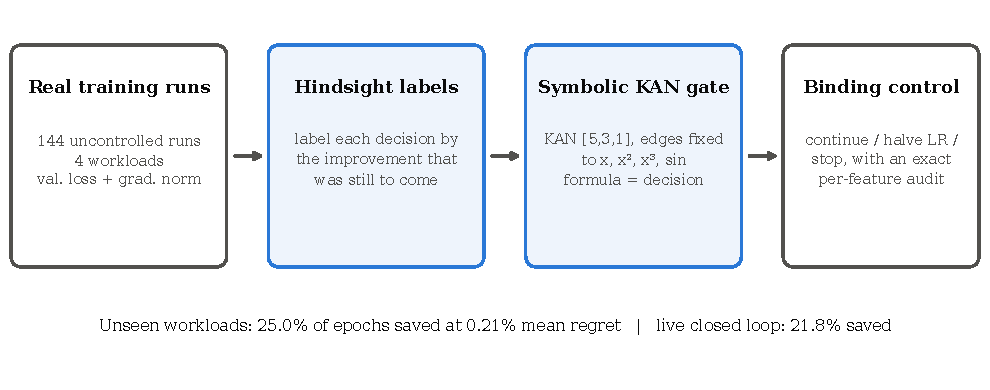
\includegraphics[width=\linewidth]{graphical_abstract.pdf}
\end{graphicalabstract}

\begin{keyword}
Kolmogorov--Arnold networks \sep early stopping \sep interpretable machine learning \sep learning-rate control \sep training orchestration \sep agentic systems
\end{keyword}
